\chapter{Protokoll\label{chapter_protokoll}}
Die Praktikumsplatine muss mit der Motorplatine kommunizieren, um das Fahrzeug in Bewegung zu setzen.
Diese Kommunikation sollte möglichst
effizient erfolgen. Die Entwicklung eines guten Protokolls ist deshalb
sehr wichtig für das gesamte System.\\
Das Vorläufer-Protokoll benutzte Zeichenketten, um Instruktionen zu übermitteln.
Dies hat zwei gravierende Nachteile. 
Zum einen nimmt das Zusammensetzen der Zeichenketten mithilfe der verfügbaren Prozessoren
sehr viel Rechenleistung in Anspruch.
Zum anderen ist durch die Verwendung der Zeichenketten die Informationsdichte der Instruktionen
nicht sehr hoch, und es fällt zusätzliche Wartezeit bei der Übermittlung an.

\section{Grundlegende Konzepte}
Da die Kommunikations-Einrichtungen der Hardware Byte-orientiert sind, wurde das
Protokoll ebenfalls Byte-orientiert aufgebaut. Im Gegensatz zu dem Vorgänger-Protokoll
werden also keine Zeichenketten benutzt, um die Informationen zu repräsentieren, sondern
nur der Wert der einzelnen Bytes.\\
Ein Befehl ist eine Folge von n Bytes, wobei n mindestens 1 und maximal der im Code
eingestellten Größe der Befehlsstruktur entspricht. 
Die maximale Länge der einzelnen eingebauten Befehle beträgt 9 Bytes.
Das erste Byte eines Befehls hat eine
besondere Bedeutung. Dieses Byte wird Kommando-Byte genannt. Das Kommando-Byte
ist in zwei Teile geteilt. Der erste Teil umfasst die 4 Bits mit der niedrigsten Wertigkeit und
wird Befehlscode genannt. Der Befehlscode spezifiziert die Art des Befehls.
Der zweite Teil beinhaltet die höchstwertigen 4 Bits. Darin werden Optionen
gesetzt, die den im Befehlscode angegebenen Befehl modifizieren. Die Kombination
von Befehlscode und Optionen legt auch die Länge des Befehls fest. Alle dem
Kommando-Byte folgende Bytes sind Parameter, wie z.B. die Geschwindigkeit der Räder.\\
Da 4 Bits für Befehlscodes zur Verfügung stehen, sind 16 verschiedene Befehle möglich.
Sechs Befehle wurden im Zuge dieser Arbeit implementiert; das würde noch Platz für
10 weitere Befehle lassen. Das Protokoll sollte allerdings noch mehr Freiheiten
für zukünftige Erweiterungen bieten, deswegen wurde einer der Befehlscodes
reserviert. Dieser reservierte Befehlscode und dessen Behandlung im Code ermöglichen
es, dass es mehr als ein Kommando-Byte geben kann. Damit ist es möglich, Befehle einfach 
hinzuzufügen, die nicht in das Schema ''ein Kommando-Byte, viele Parameter'' passen.\\
Wenn Parameter übertragen werden müssen, die mehr als ein Byte benötigen, wird zuerst
das höchstwertige Byte übertragen. Danach, absteigend nach der Wertigkeit, folgen die anderen
Bytes.\\
Durch die volle Ausnutzung der Bytes gibt es kein Protokoll-spezifisches STOP- oder START-Byte.
Das bedeutet, dass das Protokoll sich auf die Flusskontrolle der zugrunde liegenden Hardware
verlässt.

\section{Eingebaute Befehle}
Sechs Befehle und die Infrastruktur für den reservierten Befehlscode wurden implementiert.
Im Nachfolgenden werden die Befehle einzeln vorgestellt. Dabei wurde der Befehlscode bei
jedem Befehl in hexadezimaler Schreibweise als ganzes Byte dargestellt.

\subsection{Extended-Instruction - 0x00}
Dieser Befehl ist ein Platzhalter für zukünftige Befehle, die mehr als ein Kommando-Byte benötigen,
oder für den Fall, dass alle normalen Befehlscodes bereits vergeben sind. Der Befehlscode ist \textbf{0x00}.\\
Im Code werden solche Befehle mit besonderen Funktionen behandelt. Die 
parser\_\-extended\_\-order\_\-complete-Funktion ist ein Beispiel hierfür. Diese
besonderen Funktionsvarianten gibt es allerdings nur im Parser.
Nach dem Verlassen des Parsers wird eine Extended-Instruction wie ein normaler Befehl behandelt.
Die zusätzlichen Funktionen waren nötig, weil sich diese Befehle im Aufbau von normalen Befehlen stark unterscheiden.

\subsection{Control - 0x01}
Mit diesem Befehl kann das System gesteuert werden. Darunter fallen Aufgaben wie das
Reseten des gesamten Programms, das Anhalten der Befehlsausführung, und die Manipulation
der Befehls-Warteschlange. Der Befehlscode für diesen Befehl ist \textbf{0x01}. Außerdem ist der Control-Befehl
ein priorisierter Befehl, d.h. er wird bei dem nächsten Hauptschleifendurchlauf ausgeführt und nicht
an die Warteschlange angereiht.\\
Die in Tabelle \ref{protocol_control} beschriebene Bitmaske wird mit dem Befehlscode verodert
und ergibt das Kommando-Byte. Bei manchen Befehlen können mehrere Optionen zur gleichen Zeit
gewählt werden; dies ist hier nicht der Fall. Die Optionen dieses Befehls schließen sich
gegenseitig aus. Die Länge der Befehle mit vorgenanntem Befehlscode beläuft sich auf 1 Byte, sodass
lediglich das Kommando-Byte gesendet werden muss.
\begin{table}[htb]
\begin{center}
	\begin{tabularx}{\linewidth}{|l|c|c|X|}
		\hline
		\textbf{Option} & \textbf{Bitmaske} & \textbf{resultierendes} & \textbf{Beschreibung} \\
		                &                   & \textbf{Kommando-Byte}   & \\
		\hline
		\hline
		Reset 			& 0x10 				& 0x11                    & Hardware-Reset \\
		\hline
		Stop Queue		& 0x20				& 0x21                    & Der Aktuelle Befehl wird verworfen. Die Warteschlange wird angehalten, aber nicht verworfen. \\
		\hline
		Continue Queue	& 0x30				& 0x31                    & Der nächste Befehl in der Warteschlange wird ausgeführt. \\
		\hline
		Clear Queue		& 0x40				& 0x41                    & Die Warteschlange wird gelöscht. \\
		\hline
		Stop Drive		& 0x50				& 0x51                    &Befehl wird angehalten, Fahrzeug geht zum aktiven Bremsen über. \\
		\hline
	\end{tabularx}
	\caption{\label{protocol_control} Optionen des Control-Befehls}
\end{center}
\end{table}

\subsection{Query - 0x02}
Manchmal ist es wichtig, dass die kontrollierende Praktikumsplatine verschiedene Laufzeitwerte
der Motorplatine kennt. Dieser Befehl, dem der Befehlscode \textbf{0x02} zugeordnet ist, ermöglicht
es, die Geschwindigkeit der Räder, die Anzahl der Befehle in der Warteschlange und den aktuellen
Befehl abzufragen. Die Optionen schließen sich gegenseitig aus, und die Länge des Befehls beträgt
immer 1 Byte. Der Befehl ist wie der Control-Befehl ein priorisierter Befehl. Er wird also
nicht an die Warteschlange angereiht.\\
Wenn nach Senden dieses Befehls an die Motorplatine kurz darauf versucht wird, über den I2C-Bus
das Ergebnis zu lesen, kann der Fall eintreten, dass es noch nicht vorliegt.
Das geschieht besonders dann, wenn der aktuelle Befehl angefordert wurde.
In diesem Fall muss die Lese-Operation nochmals gestartet werden.\\
Die Länge des aktuellen Befehls muss mit übertragen werden, damit die Praktikumsplatine
diesen Befehl, den die Motorplatine zurückgibt, auch verwerten kann.
Es ist deshalb nötig, dass die Praktikumsplatine zwei Lese-Operationen durchführt,
wobei die erste eine Länge von einem Byte hat und außerdem spezifiziert, wie lang die zweite Antwort in Bytes ist.

\begin{table}[htb]
\begin{center}
	\begin{tabularx}{\linewidth}{|c|c|X|l|}
		\hline
		\textbf{Bitmaske} & \textbf{resultierendes} & \textbf{Beschreibung} & \textbf{Antwortlänge} \\
		                  & \textbf{Kommando-Byte}  &                       & \textbf{in Bytes}\\
		\hline
		\hline
		0x10              & 0x12                    & Geschwindigkeit des linken Rades & 1 \\
		\hline
		0x20              & 0x22                    & Geschwindigkeit des rechten Rades & 1 \\
		\hline
		0x30              & 0x32                    & Anzahl der Befehle in der Warteschlange & 1 \\
		\hline
		0x40              & 0x42                    & Aktueller Befehl & 2 - 16 \\
		\hline
	\end{tabularx}
	\caption{\label{protocol_queue} Optionen des Query-Befehls}
\end{center}
\end{table}

\subsection{Drive - 0x03}
Der am häufigsten benutzte Befehl ist der Drive-Befehl. Durch ihn werden die Räder des Fahrzeugs
in Bewegung gesetzt. Ihm ist der Befehlscode \textbf{0x03} zugeteilt, und seine Länge beträgt zwischen 3
und 7 Bytes. Im Minimalfall besteht der Befehl aus dem Kommando-Byte und je einem Byte für
die gewünschte Geschwindigkeit der einzelnen Räder. Ohne die Angabe einer Abbruchbedingung für
beide Räder würde dieser Befehl endlos laufen, oder solange, bis mithilfe des Control-Befehls
die Ausführung unterbrochen wird. Die Abbruchbedingungen werden Trigger genannt. 
Die Räder sind mit zwei Trigger-Arten ausgerüstet:
Die Positions-Trigger und die Zeit-Trigger. Die Positions-Trigger stoppen
das Rad, dem sie zugeordnet wurden, nachdem eine bestimmte Anzahl an Interrupts von dem Rad
ausgelöst wurden. Die Zeit-Trigger stoppen das Rad, nachdem die angegebene Fahrzeit erreicht
wurde. 
Dadurch kann jedes Rad für sich entweder durch keinen Trigger, durch einen Zeit-Trigger
oder durch einen Positions-Trigger beeinflusst werden.
Triggerwerte sind
2 Bytes lang und nur positiv. Die Geschwindigkeit ist 1 Byte lang und kann auch negativ sein.
Dem Kommando-Byte folgt daher das Byte für die Geschwindigkeit des linken Rades, dann
das Byte für die Geschwindigkeit des rechten. Falls Triggerwerte angegeben werden müssen,
erfolgt dies nach den Geschwindigkeitsangaben.
Man beginnt ebenfalls mit dem Triggerwert für das linke Rad, dann folgt der
Wert für das rechte.\\
Zusätzlich zu diesen Fahrmöglichkeiten gibt es einen speziellen Fahrmodus, der für
die ''Geradeaus-Fahrt'' optimiert ist. Er wird als ''Fahrt mit Differenzausgleich''
bezeichnet. Hierbei wird versucht, die Differenz beider Räder möglichst auf 0 zu
halten. Wegen der Geradeaus-Fahrt entfällt die zweite Geschwindigkeitsangabe, und 
die Bitmasken für die Trigger des rechten Rades gelten für beide Räder. Eine weitere
Bitmaske erlaubt es, den Startwert des Differenzwertes festzulegen. Dieser ist dann
der einzige Parameter, 2 Bytes lang und vorzeichenbehaftet.\\
Zur Konstruktion des Kommando-Bytes für diesen Befehl wird der Befehlscode mit der Bitmaske
für das linke und rechte Rad verodert.
Dabei ist zu beachten, dass eine der drei Möglichkeiten
ausgewählt wird, die in dem oberen Teil der Tabelle \ref{protocol_opt_drive} vorgestellt werden.
Das gilt nur, wenn keine der Bitmasken 0x30 oder 0xc0 verwendet werden.
\begin{table}[h]
\begin{center}
	\begin{tabularx}{\linewidth}{|l|l|l|X|}
		\hline
		\textbf{Byte-Anzahl} & \textbf{Option} & \textbf{Wertebereich} & \textbf{Beschreibung} \\
		\hline
		\hline
		1					 & - & -128 bis 127 & Geschwindigkeit des linken Rades \\
		\hline
		1					 & - & -128 bis 127 & Geschwindigkeit des rechten Rades\\
		\hline
		2					 & Zeit-Trigger & 0 bis 65535 &  die Fahrzeit des linken Rades (in 100 ms)\\
		\hline
		2					 & Positions-Trigger & 0 bis 65535 &  Anzahl der Ticks für die Fahrt des linken Rades\\
		\hline
		2					 & Zeit-Trigger & 0 bis 65535 &  die Fahrzeit des rechten Rades (in 100 ms)\\
		\hline
		2					 & Positions-Trigger & 0 bis 65535 &  Anzahl der Ticks für die Fahrt des rechten Rades\\
		\hline
	\end{tabularx}
	\caption{\label{protocol_para_drive} Parameter des Drive-Befehls}
\end{center}
\end{table}
\begin{table}[h]
\begin{center}
	\begin{tabularx}{\linewidth}{|p{2cm}|l|l|X|}
		\hline
		\textbf{Option} & \textbf{Bitmaske links} & \textbf{Bitmaske rechts} & \textbf{Beschreibung} \\
		\hline \hline
		Kein Trigger	& 0x00						   & 0x00						   & Endlosfahrt \\ \hline
		Zeit-Trigger	& 0x10						   & 0x40						   & zeitlich begrenzte Fahrt\\ \hline
		Positions-Trigger & 0x20					   & 0x80						   & fährt eine bestimmte Strecke \\ \hline
		Fahrt mit Differenz-Ausgleich & 0x30		   & -						   & beide Räder fahren mit derselben Geschwindigkeit geradeaus \\ \hline
		Differenz setzen & 0xc0					   	   & -						   & setzt die Differenz der Räder \\ \hline
	\end{tabularx}
	\caption{\label{protocol_opt_drive} Optionen des Drive-Befehls}
\end{center}
\end{table}
\begin{figure}[h]
 \centering
 \scalebox{0.5}{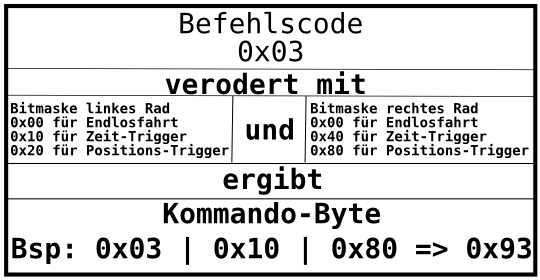
\includegraphics{pictures/drive_konzept.png}}
 \caption{\label{prot_drive_concept}Das grundlegende Konzept zur Erstellung eines Drive-Kommando-Bytes}
\end{figure}

\subsection{Advanced-Drive - 0x04}
Der Advanced-Drive-Befehl, der den Befehlscode \textbf{0x04} besitzt, verhält sich grundsätzlich
wie der normale Drive-Befehl. Er bietet allerdings mehr Möglichkeiten für den Einsatz der Trigger.
Wird der Befehl ohne Trigger
verwendet, so ist er mit dem Drive-Befehl identisch. Werden diese jedoch verwendet,
müssen für jedes Rad zwei Trigger-Werte angegeben werden. Es werden also immer Zeit-
und Positions-Trigger verwendet. Je nach gewählter Option werden sie miteinander mit einem logischen
UND oder einem logischen ODER verknüpft. So ist es möglich, Fahrbefehle
zu erteilen, die entweder eine bestimmte Strecke oder eine bestimmte Zeit fahren.
\begin{table}[h]
\begin{center}
	\begin{tabularx}{\linewidth}{|X|l|l|X|}
		\hline
		\textbf{Option} & \textbf{Bitmaske Links} & \textbf{Bitmaske Rechts} & \textbf{Beschreibung} \\
		\hline
		\hline
		Kein Trigger				& 0x00						   & 0x00						   & Endlosfahrt \\
		\hline
		Zeit-Trigger ODER Positions-Trigger	& 0x10						   & 0x40						   & Fahrt bis Erreichen eines Triggers\\
		\hline
		Zeit-Trigger UND Positions-Trigger  & 0x20						   & 0x80						   & Fahrt bis Erreichen beider Trigger\\
		\hline
	\end{tabularx}
	\caption{\label{protocol_advanced_drive} Optionen des Advanced-Drive-Befehls}
\end{center}
\end{table}

\subsection{SetPID - 0x05}
Das PID-Modul benutzt mehrere Parameter, um den Fehlerausgleich durchzuführen. Diesen
Parametern sind im Programmcode bereits Standardwerte zugewiesen worden. Es kann aber
vonnöten sein, diese Parameter anzupassen. Dafür ist der SetPID-Befehl erforderlich.
Dieser besitzt den Befehlscode \textbf{0x05}. Seine Länge beträgt immer 9 Bytes. Es müssen
alle Werte dem SetPID-Befehl übergeben werden. Jeder Wert benötigt 2 Bytes.
Die Werte können auch negativ sein. Sie werden in der Reihenfolge angegeben,
wie sie im oberen Teil der Tabelle \ref{protocol_setpid} zu finden sind.
Die genaue Auswirkung dieser Einstellungen sollte vom Benutzer in der Studienarbeit von
Timo Klingeberg \cite{STUD_TIMO} nachgelesen werden.
\begin{table}[htb]
\begin{center}
	\begin{tabular}{c}
	\begin{tabularx}{\linewidth}{|l|l|l|X|}
		\hline
		\textbf{Byte-Anzahl} & \textbf{Position} & \textbf{Wertebereich} & \textbf{Beschreibung} \\
		\hline
		\hline
		2					 & 1 & -32768 bis 32767 & \textbf{P}roportionaler Faktor\\
		\hline
		2					 & 2 & -32768 bis 32767 & \textbf{I}ntegraler Faktor\\
		\hline
		2					 & 3 & -32768 bis 32767 & \textbf{D}ifferentieller Faktor\\
		\hline
		2					 & 4 & -32768 bis 32767 & maximaler Fehlersummen-Modifikator\\
		\hline
	\end{tabularx}\\
	\\
	\begin{tabularx}{\linewidth}{|l|c|X|}
		\hline
		\textbf{Option} & \textbf{Bitmaske} & \textbf{resultierendes Kommando-Byte} \\
		\hline
		\hline
		linkes Rad	& 0x00 & 0x05 \\
		\hline
		rechtes Rad	& 0x10 & 0x15 \\
		\hline
		beide Räder & 0x20 & 0x25 \\
		\hline
	\end{tabularx}
	\end{tabular}
	\caption{\label{protocol_setpid} Parameter und Optionen des SetPID-Befehls}
\end{center}
\end{table}

\subsection{Option - 0x06}
Der Option-Befehl besitzt den Befehlscode \textbf{0x06} und hat eine Länge von 2 Bytes.
Durch ihn können bestimmte Variablen auf der Motorplatine während der Laufzeit
geändert werden. Momentan kann damit das ABS (siehe Kapitel \ref{chapter_abs}) angepasst werden. Nach dem
Kommando-Byte folgt der neue Wert der Variablen.
\begin{table}[htb]
\begin{center}
	\begin{tabularx}{\linewidth}{|l|l|l|X|}
		\hline
		\textbf{Bitmaske} & \textbf{Default} & \textbf{Wertebereich (Bytes)} & \textbf{Beschreibung} \\
		\hline
		\hline
		0x10 & 40 & 1 bis 127 (1) & Geschwindigkeitswert beim aktiven Bremsen\\
		\hline
		0x20 & 1 & 0 oder 1 (1) & Schalter zum Aktivieren der aktiven Bremsung (eine 1 bedeutet die Aktivierung)\\
		\hline
		0x30 & 1 & 0 oder 1 (1) & Schalter zum Aktivieren der aktiven Bremsung \textbf{des} Rades, das seinen Trigger erreicht hat\\
		\hline
		0x40 & 1 & 0 oder 1 (1) & Schalter zum Aktivieren der aktiven Bremsung, wenn kein Befehl bearbeitet wird\\
		\hline
	\end{tabularx}
	\caption{\label{protocol_option} Optionen des Option-Befehls}
\end{center}
\end{table}
